\documentclass{article}
\usepackage[utf8]{inputenc}
\usepackage{tikz}
\usetikzlibrary{arrows}

\def\R{{\rm R}}
\def\L{{\rm L}}
\def\LR{{\rm LR}}
\def\Rs{{\rm R}^*}
\def\M{{\rm M}}
\def\LLR{{\rm L}_2{\rm R}}
\def\MR{{\rm MR}}
\def\LRs{{\rm LR}^*}


\begin{document}

\begin{center}

\section*{Reaction Scheme Diagrams}

\vspace{0.5in}

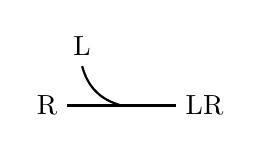
\begin{tikzpicture}[node distance=2cm,>=latex']
\node[] (R) {$\R$};
\node[right of=R] (LR) {$\LR$};
\draw [thick] (R) to node[below] {} node[above] (midwayabove) {} (LR);
\draw [thick] (LR) to (R) ;
\draw [thick] (midwayabove.south) to [bend left] +(-0.5,0.5) node[above] {$\L$};
\end{tikzpicture}

\vspace{0.5in}

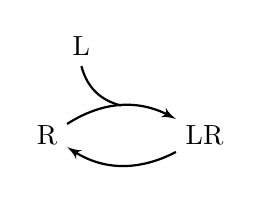
\begin{tikzpicture}[node distance=2cm,>=latex']
\node[] (R) {$\R$};
\node[right of=R] (LR) {$\LR$};
\draw [->,thick] (R)  to [bend left] node[above] (midwayabove) {} (LR);
\draw [->,thick] (LR) to [bend left] (R) ;
\draw [thick] (midwayabove.south) to [bend left] +(-0.5,0.5) node[above] {$\L$};
\end{tikzpicture}

\vspace{0.5in}

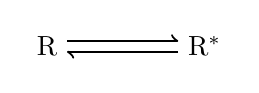
\begin{tikzpicture}[node distance=2cm]
\node (R) {$\R$};
\node[right of=R] (Rs) {$\Rs$};
\draw [-left to,thick,transform canvas={yshift=.2em}] (R) -- (Rs);
\draw [-left to,thick,transform canvas={yshift=-.2em}] (Rs) -- (R);

\end{tikzpicture}

\vspace{0.5in}


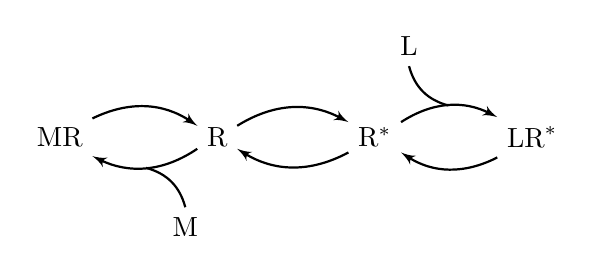
\begin{tikzpicture}[node distance=2cm,>=latex']
\node (MR) {$\MR$};
\node[right of = MR] (R) {$\R$};
\draw [->,thick] (MR) to [bend left] (R);
\draw [->,thick] (R) to [bend left]  node[above] (midwaybelow) {} (MR);
\draw [thick] (midwaybelow.south) to [bend left] +(0.5,-0.5) node[below] {$\M$};
\node[right of = R] (Rs) {$\Rs$};
\draw [->,thick] (R) to [bend left] (Rs);
\draw [->,thick] (Rs) to [bend left] (R);
\node[right of = Rs] (LRs) {$\LRs$};
\draw [->,thick] (Rs) to [bend left] node[above] (midwayabove) {} (LRs);
\draw [->,thick] (LRs) to [bend left] (Rs) ;
\draw [thick] (midwayabove.south) to [bend left] +(-0.5,0.5) node[above] {$\L$};
\end{tikzpicture}

\end{center}

\end{document}
